\chapter{Simulation, reconstruction and datasets}
\section{Simulation}
Accurate Monte Carlo simulations are needed in order to make sense of the
data and search for new physics phenomena. The physics of the collisions is
simulated by the event generators MadGraph~\cite{madgraph} and PYTHIA~\cite{fs:pythia}. Then, the propagation of the particles in the detector has to be worked out.
Two different types of simulation are used by the CMS collaboration: a
GEANT4-based~\cite{fs:geant} simulation, known as the \emph{Full
Simulation}, and a detector model with simplified geometry, response
evaluation and pattern recognition to decrease the processing time per
event, the \emph{Fast Simulation}~\cite{fs:fast.simulation}. Both the
FullSim and the FastSim were employed in the generation of the background
samples for our studies.

In the FullSim, the energy depositions in the sensitive detector volumes are converted to electronic
signals using algorithms based on the observed detector behavior, including the simulation of
electronics noise and cross-talk. In many cases, the simulated electronic parameters are identical to
those of the real electronics; the constants specifying performance, calibrations, and noise behavior
can be read from the same database used for the reconstruction of the real collision data. The output of
this stage is simulated data in a format identical to that of the real raw data read from the detector.
Further processing uses this data to simulate the formation of the L1 and
HLT decisions using the same algorithms implemented online in the CMS trigger system. The simulated
raw data that is produced is processed in a manner identical to that of the real data from
LHC collisions.

The FastSim makes a number of approximations:
\begin{description}
    \item[CMS geometry:] the FastSim describes the detector with a simplified geometry of nested cilyndrical layers. The particles are propagated from one layer to the next.
    \item[Material effects:] five effects are taken into account. These are \emph{bremsstrahlung}, photon conversion, multiple Coulomb scattering, energy loss through ionization and nuclear interactions. All of these are calculated analytically, except for nuclear interactions, since no analytical description is sufficient to describe the effect. Cross sections are taken from the PDG and the kinematics are derived from single particle collisions saved beforehand.
    \item[Track reconstruction:] the reconstruction is not usually part of the simulation. The FastSim includes it because, given the low fake rate in the reconstruction, it is possible to emulate it at a lower computational cost. Only the hits of the simulated track are used to make a track candidate. 
    \item[Muons:] muons are propagated through the tracker and calorimeters with average energy loss, then $dE/dx$ and multiple scattering in the iron yokes of the muon chambers are computed. Muon simulated hits are produced in all sections of the muon systems.
    \item[Calorimeters:] electron showers in the ECAL are simulated with the Grindhammer~\cite{fs:grindhammer} parametrization. Photons undergo pair conversions based on the number of radiation lengths they have traversed. Detector effects such as energy leakage into the crystal gaps and into the HCAL are included, as well as electronic noise. Shower simulation in the HCAL is similar, with different types of particles parametrized from FullSim results.
\end{description}

\section{The reconstruction of physics objects}
The particle flow~\cite{pf:particle.flow} (PF) event reconstruction aims at reconstructing and identifying all stable particles in the event. The essential idea is to analyse the event combining the information from all the available subdetectors in an optimal way.

The CMS detector, with its large silicon tracker and its extremely precise electromagnetic calorimeter, appears to be ideally suited for this purpose. The fundamental building bricks of the PF reconstruction are charged particle tracks, ECAL and HCAL clusters and muon tracks. These must be delivered with a high efficiency and low fake rate even in high-density environments like jets. A jet is a collection of particles resulting from the decay of a quark or gluon and emitted in the direction of the primary particle. 

Reconsider the design of the detector in figure~\ref{fig:cms_transverse}. The logic you use to
interpret this diagram is akin to that employed by the PF.
An ECAL cluster not linked to any track is a photon, an ECAL and HCAL cluster matched to a track gives a charged hadron, while an HCAL cluster without a track identifies a neutral hadron. Electrons are basically ECAL-only clusters linked to a track. Muons are by far the easiest particles to recognize.

From these basic elements, composite objects can be reconstructed, such as
$\tau$ leptons from their decay products, jets and
missing transverse energy from all the particles in the event.

Quality requirements are needed in the reconstruction of the physics
objects: thousands of particles are created in each event and their tracks
can overlap.
The quality selections are the result of detailed studies by the CMS
collaboration, aiming for the best compromise between purity and efficiency.
These recommendations are described in the following paragraphs.

\subsection{Muon reconstruction}
Muons are not stopped inside the CMS detector and leave only a tiny fraction
of their energy in the calorimeters. The information from the tracking
system and the muon chambers is exploited for their reconstruction.
The two systems are used independently in a first phase, where two
algorithms are used:
\begin{description}
    \item[The global muon reconstruction], or the \emph{outside-in}
        approach, starts from a segment in the drift tubes or cathode strip
        chambers and extrapolates the seed layer by layer up to the
        tracker. If a matching track is found in the tracking system, the
        information from both tracks is combined to improve the resolution.
    \item[The tracker muon reconstruction], or the \emph{inside-out} method,
        extrapolates a track from the inner system to the muon chambers. The
        small energy loss due to interactions with the material of the
        magnets and calorimeters is taken into account, as well as an
        uncertainty arising from the possibility of multiple scattering.
\end{description}
The recommended selection requires these two algorithms to agree, as this
improves the resolution for high-$\pt$ muons
(figure~\ref{fig:muon_resolution}).

\begin{figure}[htb]
    \centering
    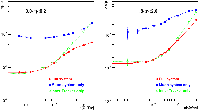
\includegraphics[width=\textwidth]{images/pdf/muon_momentum_resolution}
    \caption{Muon momentum resolution as a function of \pt in regions with
    different pseudorapidity. The blue squares are for the muon system only,
the green circles for the inner tracker only, and the red circles for the
combined reconstruction}
    \label{fig:muon_resolution}
\end{figure}

One of the most important observables for the muon candidates is the
\emph{relative isolation}. It indicates the amount of energy collected in
the vicinity of the muon, by summing the contributions from the tracking
system, the ECAL and the HCAL, divided by the \pt of the muon.
The sum runs over all deposits within a cone of radius $\Delta R = 0.3$
centred on the muon track, as illustrated in figure~\ref{fig:muon_isolation}.

\begin{figure}[htb]
    \centering
    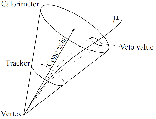
\includegraphics[width=.5\textwidth]{images/pdf/muon_isolation}
    \caption{Illustration of the isolation observable.}
    \label{fig:muon_isolation}
\end{figure}

\subsection{Electron reconstruction}
The tracks in CMS are reconstructed assuming that the particle is a muon.
Coulomb scattering is the dominant effect on muons crossing material and its
impact is modelled by gaussian fluctuations. This approach fails with
electrons because of the highly non-gaussian \emph{bremsstrahlung} emission. A
customized track reconstruction was developed for electrons, where the hits
are fitted using a \emph{gaussian sum filter} (GSF)~\cite{pf:gsf.tracks},
\ie the \emph{bremsstrahlung} emission is modelled by a superposition of
gaussian functions. However, this more sophisticated analysis demands more CPU power, at the order of a few hundreds milliseconds per track, and can be run only on a limited number of seeds.

The standard strategy to seed GSF tracks, hereafter called ECAL-driven seeding, heavily relies on
the ability to gather into one single \emph{supercluster} the entire energy deposit of the electron. 
The algorithm consists of three steps. First, cluster seeds are identified
as local energy maxima above a given energy. Secondly, the seeds are
grown by connecting cells with at least one side in common with
a cell already in the cluster, and with an energy in excess of a given
threshold. These thresholds are equivalent to two standard deviations of the electronic noise in the calorimeter, that is $\unit[80]{MeV}$ in the ECAL barrel, up to $\unit[800]{MeV}$ in the HCAL. Finally cluster energies and positions are determined from those clusters.

This implies collecting the electron and the \emph{bremsstrahlung} photons energy deposits, 
which leads to clusters very extended along the azimuthal direction. 
This approach, which is efficient for isolated and high $\pt$ electrons has unfortunately 
a limited efficiency in jets because the super-cluster collects 
additional contributions from other particles.

In contrast with this ECAL-driven approach, the strategy developed for the Particle Flow~\cite{pf:electron.reconstruction} starts from
the tracks and can be explained with two extreme examples. 
When the \emph{bremsstrahlung} emission is negligible, the electron
trajectory is determined with good precision by
the standard tracking algorithm, and the track can be reconstructed up to the ECAL internal
surface where it can be matched with the closest cluster. 
The momentum of the track can then be compared with the corresponding cluster energy, 
forming the $E/p$ observable. If it is close to unity the track is selected to be then re-reconstructed
with the GSF algorithm. On the contrary, if the electron loses a substantial fraction of its energy by \emph{bremsstrahlung} emission, the characteristics of the track are exploited. Indeed, either the pattern recognition manages
to accommodate for the changes of curvature, and the fitted track $\chi^2$ is usually large, or
it cannot follow the electron trajectory and the track is short.  
Electron tracks are then selected based on the attempt made by the standard algorithm to reconstruct it. 

The tracker-driven seeding developed for the PF reaches a 80\% efficiency in the barrel with a 10\% probability
to select wrongly a pion, with an acceptable CPU consumption; a more sophisticated treatment described below 
is further applied to reject fakes at the final identification level. 
In addition, this new algorithm improves the overall seeding efficiencies for isolated electron in CMS by 15\% at \unit[5]{GeV} with respect to the standard ECAL-driven seeding. 

\begin{figure}[htb]
    \centering
    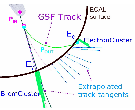
\includegraphics[width=.5\textwidth]{images/pdf/electron_reconstruction}

    \caption{An illustration of the \emph{bremsstrahlung} recovery
algorithm.}
    \label{fig:electron_reconstruction}
\end{figure}

The procedure to collect all the calorimeter energy deposits, \ie, the \emph{bremsstrahlung} recovery, is
driven by the GSF track (figure~\ref{fig:electron_reconstruction}). For each tracker layer, where 
the material is mainly localized, a \emph{bremsstrahlung} photon emission is sought by computing a straight-line
extrapolation, tangent to the track, up to the ECAL. If it matches a cluster, not already linked
to a track, this cluster is selected as part of the electron. 
This procedure allows between 96\% and 99\% of the energy deposited in the ECAL to be collected.

The relative isolation is defined with the same method already described for
the muons.

The charge of the electrons can be measured in three ways:
\begin{description}
    \item[The GSF track] whose curvature in the magnetic field of the
        detector defines the sign of the charge of the electron.
    \item[The CTF track] algorithm for the reconstruction of the
        tracks. It accounts for multiple scattering with Kalman filter
        techniques~\cite{springerlink:10.1140/epjc/s10052-006-0175-5}. The
        curvature of this track is another measurement of the charge.
    \item[Supercluster relative position] the relative position of the track seed
        and the largest deposition in the ECAL provides an indipendent
        estimate of the electric charge.
\end{description}
Requiring these three methods to agree strongly decreases the probability of
a charge mismeasurement. This is particularly important for our analysis,
since the production of opposite-sign electrons is very abundant in Standard
Model processes, and the accurate identification of the charge of the
electrons almost eliminates these contributions.

Electrons can also be created from the conversion of an energetic photon.
These are rejected if one of the following occurs:
\begin{description}
    \item[At least one missing hit] in the tracker. Photons are neutral, so they
        usually miss hits in one or more layers.
    \item[Track distance] $< \unit[0.02]{cm}$. An electron coming from a
        conversion has a partner positron track. If an oppositely charged
        track is found within this distance, the electron is rejected.
    \item[$\Delta \cot \theta < 0.02$]. A geometrical variable also related
        to the partner track: $\theta$ is the angle between the two tracks
        in the $yz$ plane.
\end{description}
